%\documentclass[portrait,final,a0paper]{baposter}
\documentclass[a0paper,portrait,final]{baposter}
% Usa a4shrink for an a4 sized paper.

\tracingstats=2

\usepackage{calc}
\usepackage{graphicx}
\usepackage{amsmath}
\usepackage{amssymb}
\usepackage{relsize}
\usepackage{multirow}
\usepackage{bm}

\usepackage{graphicx}
\usepackage{multicol}

\usepackage{pgfbaselayers}
\pgfdeclarelayer{background}
\pgfdeclarelayer{foreground}
\pgfsetlayers{background,main,foreground}

\usepackage{times}
\usepackage{helvet}
%\usepackage{bookman}
\usepackage{palatino}

\newcommand{\captionfont}{\footnotesize}

\selectcolormodel{cmyk}

\graphicspath{{images/}}


%%%%%%%%%%%%%%%%%%%%%%%%%%%%%%%%%%%%%%%%%%%%%%%%%%%%%%%%%%%%%%%%%%%%%%%%%%%%%%%%
%%%% Some math symbols used in the text
%%%%%%%%%%%%%%%%%%%%%%%%%%%%%%%%%%%%%%%%%%%%%%%%%%%%%%%%%%%%%%%%%%%%%%%%%%%%%%%%
% Format 
\newcommand{\Matrix}[1]{\begin{bmatrix} #1 \end{bmatrix}}
\newcommand{\Vector}[1]{\Matrix{#1}}
\newcommand*{\SET}[1]  {\ensuremath{\mathcal{#1}}}
\newcommand*{\MAT}[1]  {\ensuremath{\mathbf{#1}}}
\newcommand*{\VEC}[1]  {\ensuremath{\bm{#1}}}
\newcommand*{\CONST}[1]{\ensuremath{\mathit{#1}}}
\newcommand*{\norm}[1]{\mathopen\| #1 \mathclose\|}% use instead of $\|x\|$
\newcommand*{\abs}[1]{\mathopen| #1 \mathclose|}% use instead of $\|x\|$
\newcommand*{\absLR}[1]{\left| #1 \right|}% use instead of $\|x\|$

\def\norm#1{\mathopen\| #1 \mathclose\|}% use instead of $\|x\|$
\newcommand{\normLR}[1]{\left\| #1 \right\|}% use instead of $\|x\|$

%%%%%%%%%%%%%%%%%%%%%%%%%%%%%%%%%%%%%%%%%%%%%%%%%%%%%%%%%%%%%%%%%%%%%%%%%%%%%%%%
% Multicol Settings
%%%%%%%%%%%%%%%%%%%%%%%%%%%%%%%%%%%%%%%%%%%%%%%%%%%%%%%%%%%%%%%%%%%%%%%%%%%%%%%%
\setlength{\columnsep}{1.9em}
\setlength{\columnseprule}{0.0mm}


%%%%%%%%%%%%%%%%%%%%%%%%%%%%%%%%%%%%%%%%%%%%%%%%%%%%%%%%%%%%%%%%%%%%%%%%%%%%%%%%
% Save space in lists. Use this after the opening of the list
%%%%%%%%%%%%%%%%%%%%%%%%%%%%%%%%%%%%%%%%%%%%%%%%%%%%%%%%%%%%%%%%%%%%%%%%%%%%%%%%
\newcommand{\compresslist}{%
\setlength{\itemsep}{1pt}%
\setlength{\parskip}{0pt}%
\setlength{\parsep}{0pt}%
}


%%%%%%%%%%%%%%%%%%%%%%%%%%%%%%%%%%%%%%%%%%%%%%%%%%%%%%%%%%%%%%%%%%%%%%%%%%%%%%
%%% Begin of Document
%%%%%%%%%%%%%%%%%%%%%%%%%%%%%%%%%%%%%%%%%%%%%%%%%%%%%%%%%%%%%%%%%%%%%%%%%%%%%%

\begin{document}

%%%%%%%%%%%%%%%%%%%%%%%%%%%%%%%%%%%%%%%%%%%%%%%%%%%%%%%%%%%%%%%%%%%%%%%%%%%%%%
%%% Here starts the poster
%%%---------------------------------------------------------------------------
%%% Format it to your taste with the options
%%%%%%%%%%%%%%%%%%%%%%%%%%%%%%%%%%%%%%%%%%%%%%%%%%%%%%%%%%%%%%%%%%%%%%%%%%%%%%
% Define some colors
\definecolor{silver}{cmyk}{0,0,0,0.3}
%\definecolor{coral}{cmyk}{0,0.5,0.69,0.0}
\definecolor{coral}{cmyk}{0,0.58,0.69,0.0}
\definecolor{lightcoral}{cmyk}{0,0.48,0.59,0.0}
\definecolor{black}{cmyk}{0,0,0.0,1.0}
\definecolor{red}{rgb}{1,0,0}
\definecolor{darkYellow}{cmyk}{0,0,1.0,0.5}
\definecolor{darkSilver}{cmyk}{0,0,0,0.1}
\definecolor{darksalmon}{cmyk}{0,0.36,0.48,0.09}
\definecolor{salmon5}{cmyk}{0,0.41,0.41,0.56}

\definecolor{lightercoral}{cmyk}{0,0.25,0.25,0}
%\definecolor{lightercoral}{cmyk}{0,0.40,0.47,0.08}
\definecolor{apricot}{cmyk}{0.0,0.36,0.57,0.02}
\definecolor{lightestapricot}{cmyk}{0,0,0.05,0.0}

%%
\typeout{Poster Starts}
%\background{
%  \begin{tikzpicture}[remember picture,overlay]%
    %\draw (current page.north west)+(-2em,2em) node[anchor=north west] {\includegraphics[height=1.1\textheight]{silhouettes_background}};

%  \end{tikzpicture}%
%}

\newlength{\leftimgwidth}
\begin{poster}%
  % Poster Options
  {
  % Show grid to help with alignment
  grid=no,
  % Column spacing
  colspacing=1.4em,
  % Color style
%  bgColorOne=white,
%  bgColorOne=darksalmon,
  bgColorOne=white,
  bgColorTwo=darksalmon,
  %bgColorThree=red,
  borderColor=red,
  %headerColorOne=white,
  headerColorOne=lightcoral,
  headerColorTwo=darksalmon,
  headerFontColor=white,
  boxColorOne=lightercoral,
  boxColorOne=white,
  boxColorTwo=lightercoral,
  % Format of textbox
  textborder=roundedleft,
  %textborder=rectangle,
  % Format of text header
  eyecatcher=yes,
  headerborder=open,
  headerheight=0.09\textheight,
  headershape=roundedright,
  headershade=shade-tb,
  headerfont=\Large\textsf, %Sans Serif
  boxshade=plain,
  textfont={\sf },
  background=shade-tb,
  %background=plain,
  linewidth=2pt,
  columns=4
  }
  {
    \makebox[15em][l]{%
      %\begin{minipage}{8em}
        
\includegraphics[height=.08\textwidth]{acmlogo.pdf}
      %\end{minipage} 
    }
   }
  {V4VSockets: low overhead intra-node communication in Xen}
  {A. Nanos, S. Gerangelos, I. Alifieraki and N. Koziris\\ \{ananos,sgerag,ialif,nkoziris\}@cslab.ece.ntua.gr}
  {   \makebox[15em][r]{%
      \begin{minipage}{13em}
        %\vfill
        
\includegraphics[height=4em]{cslab_logo.pdf}
       \end{minipage}}
    %\makebox[5em][r]{% 
\includegraphics[height=5.0em]{ntua_logo.pdf} }
   }

%%%%%%%%%%%%%%%%%%%%%%%%%%%%%%%%%%%%%%%%%%%%%%%%%%%%%%%%%%%%%%%%%%%%%%%%%%%%%%
%  \headerbox{Motivation}{name=motivation,column=0,row=0, span=1}{
%%%%%%%%%%%%%%%%%%%%%%%%%%%%%%%%%%%%%%%%%%%%%%%%%%%%%%%%%%%%%%%%%%%%%%%%%%%%%%

%Intra-node communication suffers from severe overheads mostly due to:
%\begin{itemize}
%\item inefficient data paths
%\item packet handling
%\end{itemize}
%}
%%%%%%%%%%%%%%%%%%%%%%%%%%%%%%%%%%%%%%%%%%%%%%%%%%%%%%%%%%%%%%%%%%%%%%%%%%%%%%%
 \headerbox{I/O Path in a Generic Xen environment}{name=xenpath,row=0,column=0, span=4}{
%%%%%%%%%%%%%%%%%%%%%%%%%%%%%%%%%%%%%%%%%%%%%%%%%%%%%%%%%%%%%%%%%%%%%%%%%%%%%%%
\begin{multicols}{2}

%\hspace{0.5em}
%\begin{figure}
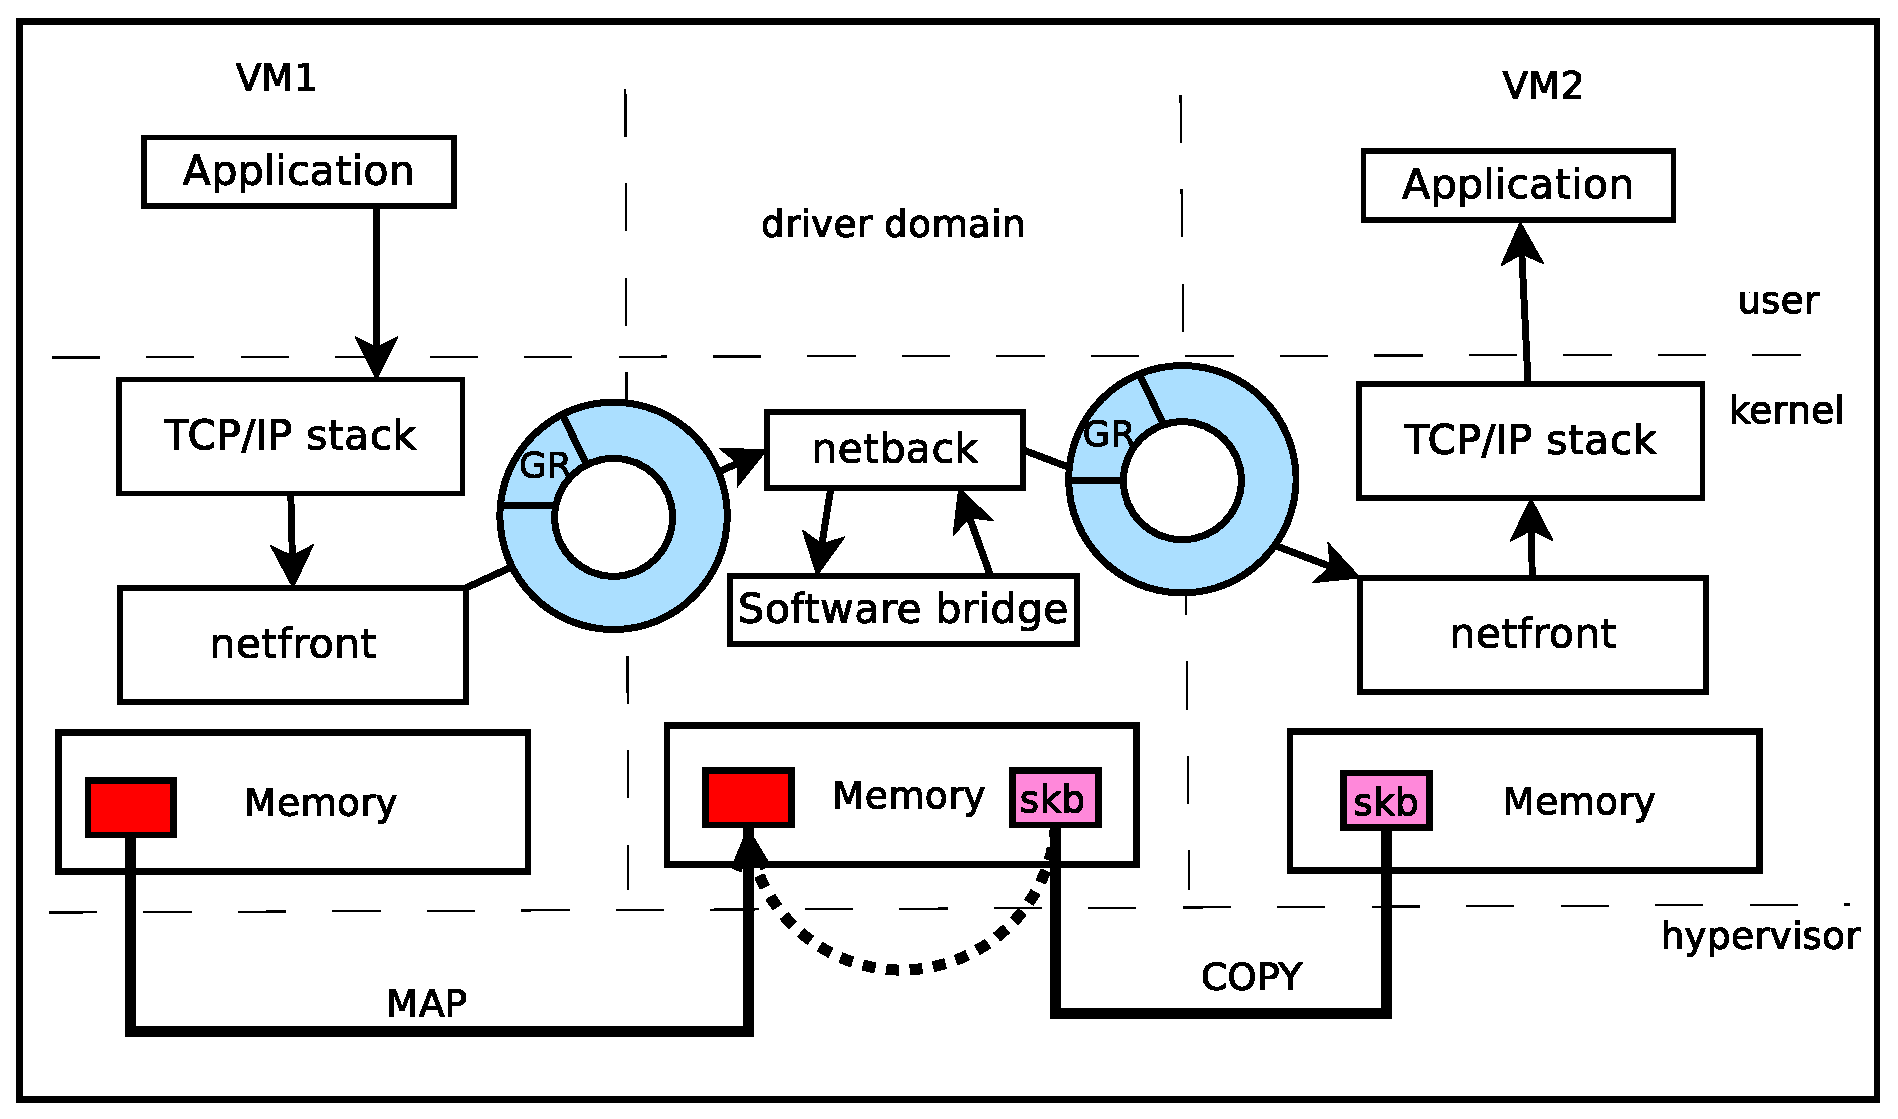
\includegraphics[width=\linewidth]{figures/netfront_netback.eps}
%\end{figure}
Intra-node communication suffers from severe overheads:
\begin{multicols}{2}
\setlength{\columnsep}{0.9em}
\setlength{\columnseprule}{0.0mm}
$\Rightarrow$ inefficient data paths

$\Rightarrow$ driver domain handles packet forwarding

V4VSockets is built as a full-stack protocol framework that supports
p2p communication between VMs. %We bypass the intermediate
\end{multicols}


%\hspace{0.5em}\scalebox{.96}{
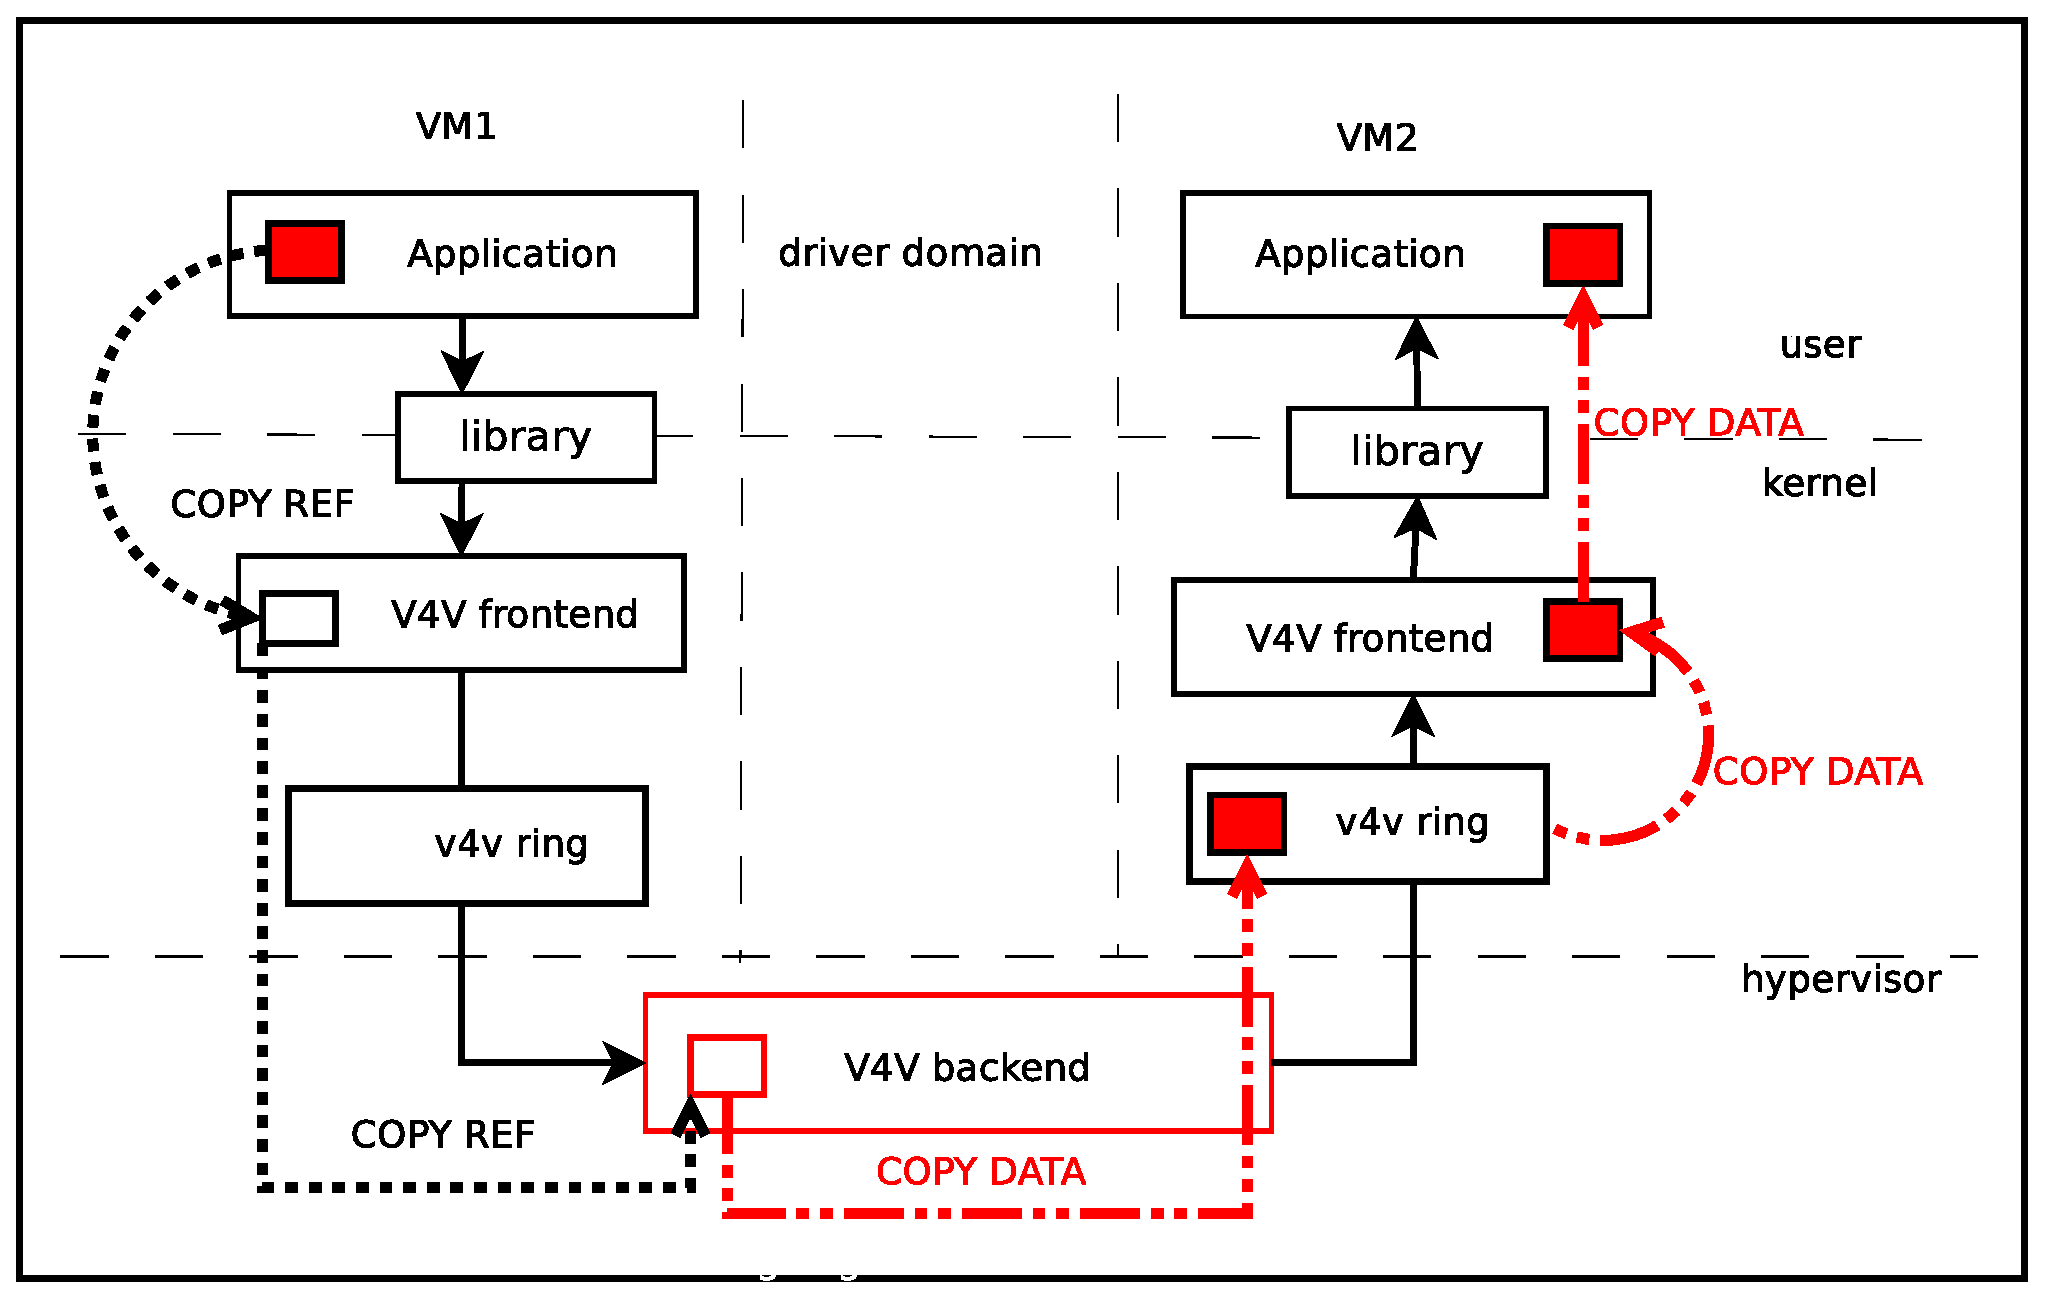
\includegraphics[width=\linewidth]{figures/v4vsockets.eps}
%}
%\includegraphics[width=.5\linewidth]{}
%layer and use the hypervisor as the control \emph{and} the data plane. 

$\Rightarrow$ \emph{Application layer}: the socket interface.

$\Rightarrow$ \emph{Transport layer}: VM kernel driver.

$\Rightarrow$ \emph{Network/Link layer}: the hypervisor, providing encapsulation of upper-layer messages to V4V messages, and packet delivery.

\end{multicols}
\vspace{.5em}
}

%%%%%%%%%%%%%%%%%%%%%%%%%%%%%%%%%%%%%%%%%%%%%%%%%%%%%%%%%%%%%%%%%%%%%%%%%%%%%%
  \headerbox{Key features}{name=contribution,column=0,span=1, below=xenpath}{
%%%%%%%%%%%%%%%%%%%%%%%%%%%%%%%%%%%%%%%%%%%%%%%%%%%%%%%%%%%%%%%%%%%%%%%%%%%%%%
V4VSockets\footnote{https://github.com/HPSI/v4v}, is an efficient,
socket-compliant, high performance intra node communication framework.

V4VSockets features:
\begin{flushleft}
$\Rightarrow$ optimized data path. Data are copied from~/~to the VM kernel memory
without the need to share pages between VMs.

$\Rightarrow$ no intermediary VM (driver domain), so no scheduling implications are involved. 

$\Rightarrow$ no security implications, data cross the hypervisor and either get dropped or pushed forward through V4V semantics. %handled through the hypervisorintermediary VM (driver domain), so no scheduling implications are involved. 

$\Rightarrow$ ultra low latency and high-bandwidth.
%$\Rightarrow$ V4VSockets preliminary evaluation, using generic micro-benchmarks versus conventional communication paths. V4VSockets outperforms the
%generic method of intra-node communication and scales efficiently with a large
%number of VMs both in terms of throughput as well as latency.

%$\Rightarrow$ real-life use case: we deploy an HPC application
%stencil over rCUDA, a remote GPU execution stack over V4VSockets.
\end{flushleft}

\vspace{1em}
}


%%%%%%%%%%%%%%%%%%%%%%%%%%%%%%%%%%%%%%%%%%%%%%%%%%%%%%%%%%%%%%%%%%%%%%%%%%%%%%%%
%% \headerbox{Acknowledgements}{name=acknowledgements,column=0,above=bottom}{
%%%%%%%%%%%%%%%%%%%%%%%%%%%%%%%%%%%%%%%%%%%%%%%%%%%%%%%%%%%%%%%%%%%%%%%%%%%%%%%%
%%  \small
%%%  \hspace{1em}
%%   The authors would like to thank Nikos Nikoleris, Elisavet Kozyri and Stratos Psomadakis for their usefull contributions to this work.
%%\vspace{0.5em}
%%  }
%
%%%%%%%%%%%%%%%%%%%%%%%%%%%%%%%%%%%%%%%%%%%%%%%%%%%%%%%%%%%%%%%%%%%%%%%%%%%%%%%
 \headerbox{Ping-pong benchmark (single pair of VMs and up to 16 VMs)}{name=results,column=1,span=3,below=xenpath}{

\begin{multicols}{2}
\hspace{0.5em}\scalebox{.800}{
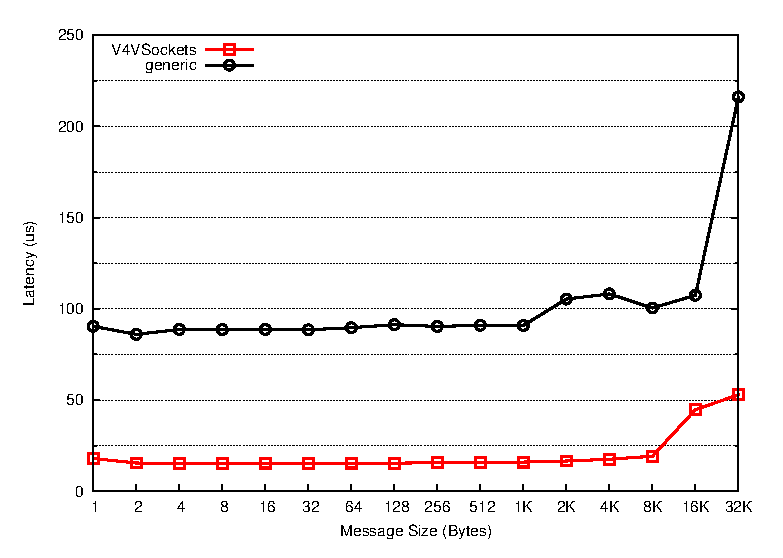
\includegraphics[width=\linewidth]{figures/v4v_lat.eps}}

\hspace{0.5em}\scalebox{.800}{
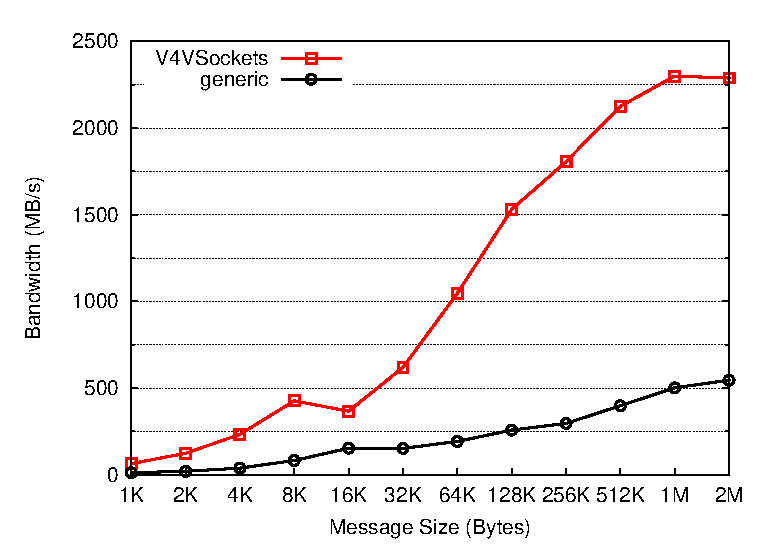
\includegraphics[width=\linewidth]{figures/v4v_bw.eps}}

\hspace{0.5em}\scalebox{.900}{
\includegraphics[width=\linewidth]{figures/new_stream_bw_scale.eps}}


V4VSockets improves the latency for small messages by 81\% compared to the
generic case. 

%\begin{multicols}{2}

V4VSockets outperforms the default case for communication. V4VSockets is able
to achieve 2299 MB/s, 4.5x better than the split driver, which performs poorly
at 501 MB/s for 1 MB messages.

The aggregate throughput achieved by V4VSockets is shown below -- we are able to reach more than half of the system's memory bandwidth%\footnote {We
%performed a stream microbenchmark and measured 27 GB/s as the maximum memory
%bandwidth.}, 
bringing memory-copy-like bandwidth measurements to VM--to--VM message exchange.

\end{multicols}

}

\headerbox{GPU stencil performance through rCUDA}{name=gpu,column=0,span=4,below=results}{
\begin{multicols}{3} 

\hspace{0.5em}\scalebox{.990}{
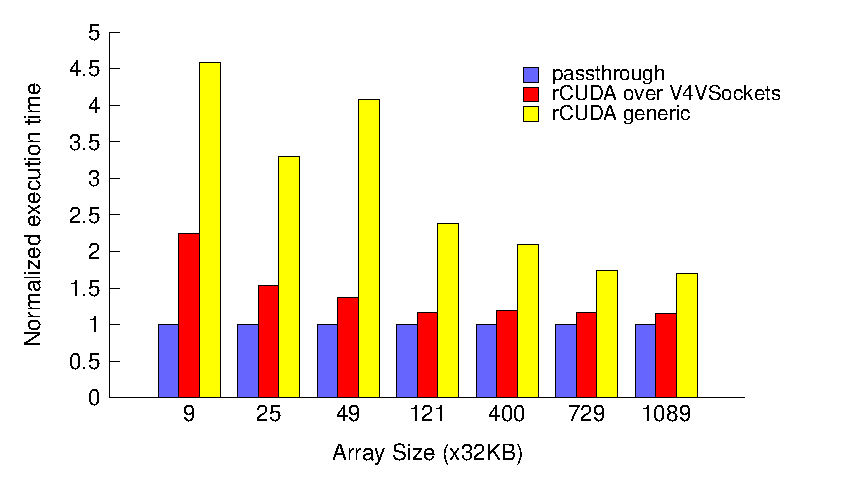
\includegraphics[width=\linewidth]{figures/total_cublas_time.eps}
}

\hspace{0.5em}\scalebox{.990}{
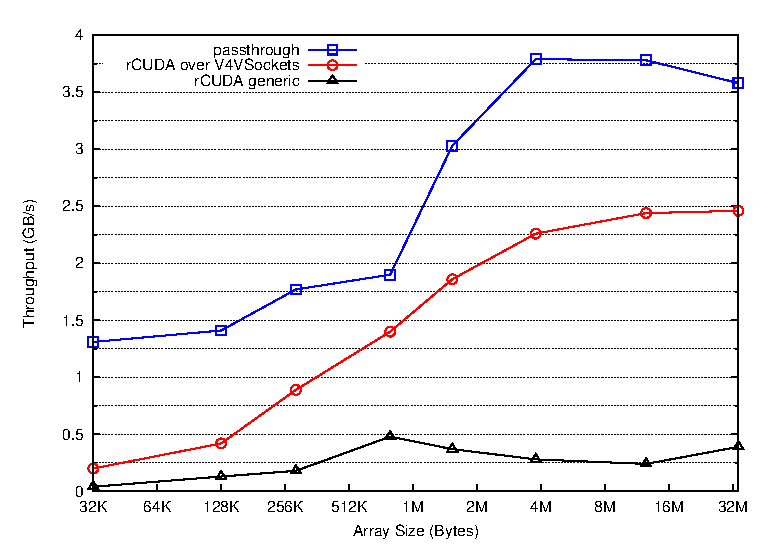
\includegraphics[width=\linewidth]{figures/matrixA_cublas_throughput.eps}
}

This experiment includes the following procedure: two copies of the input
matrices from node's main memory to GPU device memory, the product execution on
the GPU and finally one copy of the output matrix back to main memory. %We plot the
%normalized time of execution of the matrix-matrix product benchmark. 
%is
%depicted in the Figure on the left.
%\begin{multicols}{2}
%\hspace{0.5em}\scalebox{.990}{
%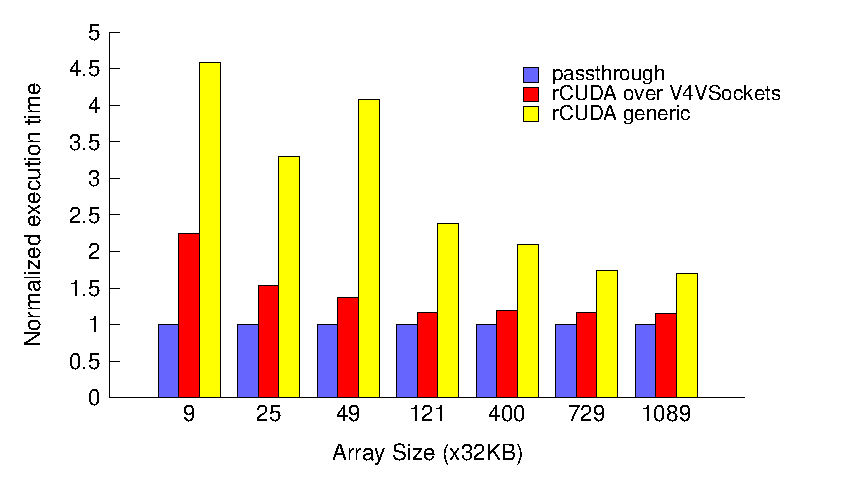
\includegraphics[width=\linewidth]{figures/total_cublas_time.eps}}
To elaborate more on the impact of V4VSockets to the improvement in the
execution time, we plot the time needed to copy one of the input
matrices from the machine's main memory to the GPU device memory. (essentially
this is a \texttt{cudamemcpy()} call).
\end{multicols}

%We observe that the peak throughput is 3.79 GB/s in our baseline experiment,
%while the respective throughput in the remote V4VSockets case is 2.46 GB/s.
%However, for a matrix size of 34 MB (2112 x 4224 float type elements)
%V4VSockets outperforms the generic case by a factor of 7 (0.35 GB/s).
%\end{multicols}

\vspace{1em}
}
\headerbox{Acknowledgments}{name=acks,column=0,span=4,above=bottom}{
The authors would like to thank the members of CSLab for the stimulating
conversations that lead to this work, especially Dr George Goumas, Dr
Konstantinos Nikas and Nikela Papadopoulou. Additionally, many thanks to the
anonymous reviewers for their useful comments and suggestions.
\vspace{1em}
}

\end{poster}

\end{document}
